%% ===================================================================
%%  When Does Adapting the Meta-Parameter Pay?
%%  Minimal governors, structural limits, and an executable audit
%%  ------------------------------------------------------------------
%%  Compile:  latexmk -pdf main.tex   (or two passes of pdflatex+bibtex)
%% ===================================================================
\documentclass[journal]{IEEEtran}

\usepackage[T1]{fontenc}
\usepackage[utf8]{inputenc}
\usepackage{amsmath,amssymb,amsthm}
\usepackage{graphicx}
\usepackage{booktabs}
\usepackage{array}
\usepackage{xcolor}
\usepackage{url}
\usepackage[colorlinks=true,linkcolor=black,citecolor=black,urlcolor=blue]{hyperref}
\usepackage{cite}

\graphicspath{{figs/}}

\newtheorem{proposition}{Proposition}
\newtheorem{lemma}{Lemma}
\theoremstyle{definition}
\newtheorem{observation}{Observation}
\newtheorem{remark}{Remark}

\newcommand{\Rset}{\mathbb{R}}
\newcommand{\simplex}{\Delta}
\newcommand{\vstar}{V^\star}
\newcommand{\Ja}{J_a}

\begin{document}

\title{When Does Adapting the Meta-Parameter Pay?\\
Minimal Governors and Structural Limits for\\
Weight- and Horizon-Governed MPC}

\author{V\'ictor~Valdivieso$^{\,a}$,
        Francisco~G.~Montoya$^{\,a}$,
        Alejandro~Campa-Pinto$^{\,b}$,
        and~Francisco~Manuel~Arrabal-Campos$^{\,a,*}$%
\thanks{$^{a}$Department of Engineering, Research Centre CIAIMBITAL,
University of Almer\'ia, 04120 Almer\'ia, Spain.}%
\thanks{$^{b}$Department of Computer Science and Electronics, Universidad de
la Costa, Barranquilla 080002, Colombia.}%
\thanks{$^{*}$Corresponding author (e-mail: fmarrabal@ual.es).}%
\thanks{Every numerical claim below is regenerated by archived scripts. The
defects found during four rounds of adversarial review of this work --- five
of them serious enough to invert a conclusion --- are each encoded as a
regression assertion in an executable audit suite distributed with the code:
\url{https://github.com/fmarrabal/limits-horizon-governed-mpc}.}}

\maketitle

\begin{abstract}
A slow outer loop that retunes an inner model predictive controller --- its
scalarization weight, or its prediction horizon --- is an appealing idea, and
we set out to make an elaborate version of it work: a second-order wave field
on the interconnection graph, transporting each subsystem's difficulty to its
neighbours. It lost in every physically grounded arena we built. What replaces
it is sharper than a negative result. First, two minimal governors that do pay.
In a chain with a physically travelling disturbance, an \emph{affine} delay
line --- per-hop delay minus a constant anticipation term --- recovers $91\%$
of an acausal clairvoyant reference --- bootstrap $95\%$ interval $[84.9,103.9]$,
which contains $100\%$ --- and cuts closed-loop cost by $12.4\%$ against the best
possible local detector; the field, a shaped filter, and the proportional delay
family that most designs default to are all significantly worse, and the
missing constant term is precisely why. In a fleet of loops sharing one
embedded controller under a hard computation budget, a governor that requests
the maximum horizon \emph{only} when the relaxed-dynamic-programming
certificate breaks, and decays slowly otherwise, beats the best fixed horizon
at equal \emph{spent} computation by up to $6\%$ --- at every
budget that binds when disturbances are independent, and at 4 of eight
budgets under a perfectly correlated front (Holm-adjusted). A decomposition into
its two mechanisms shows them to be complementary rather than cumulative:
cross-loop allocation pays only when disturbances are independent, temporal
adaptation only under a common front --- where nothing can be reallocated but
the moment to spend is well defined --- and each is neutral or harmful in the
other's regime. Second, structural limits that explain why
nothing more elaborate could win: amplitude-scale invariance of the optimal
meta-parameter, the linear-time-invariance of the graph field, the DC
cross-gain of its forcing, and a quantization-limited reach law. Third, the part most
likely to be useful beyond our own problem: five experimental leaks, two
acausal, two of accounting, one of channel, every one of which inverted a
conclusion of ours before adversarial review caught it, together with the
cheap executable tests that now keep each of them out.
\end{abstract}

\begin{IEEEkeywords}
Predictive control, adaptive horizon, resource-aware control, distributed
control, experimental methodology, negative results.
\end{IEEEkeywords}

% ====================================================================
\section{Introduction}
% ====================================================================
\IEEEPARstart{M}{odel} predictive control exposes a handful of design
quantities that are usually chosen once and then frozen: how much one objective
matters relative to another, how far ahead to predict, how hard to push soft
constraints. Letting these \emph{meta-parameters} vary online, driven by some
measured indicator of how hard the current situation is, is a natural thing to
want, and adaptive-horizon MPC, resource-aware MPC and priority scheduling all
do a version of it. A distributed version suggests itself just as readily:
couple the meta-parameters of neighbouring subsystems through a diffusion or
wave operator on the interconnection graph, so that one subsystem's decision
reaches the others without anyone having to negotiate.

We set out to make that work, across six arenas built for the purpose. The
elaborate governor won in exactly one of them --- a synthetic bench whose
priority signal had no physical origin, which is why we do not count it --- and
in none of the physically grounded ones. This paper reports what survived
instead, and it turned out to be more useful than the idea we started with.

The first thing that survived is a pair of \emph{minimal} governors that
genuinely pay, each beating not only its elaborate rivals but the natural
simple ones, and each for a reason that can be stated in one sentence. In a
transport-coupled chain, upstream information is worth $12.4\%$ of closed-loop
cost, and the mechanism that captures it is an affine delay line: what matters
is that every node receives its warning with the \emph{same} anticipation,
which a proportional delay cannot provide and a constant term can. In a fleet
of loops sharing one embedded controller, governing the horizon is worth up to
$7\%$ at equal spent computation, and the governor that achieves it is
simply a detector of certificate violation behind a slow leak: two effective
parameters. In both cases everything more sophisticated, including the field we
were defending, is statistically no better or significantly worse.

The second thing that survived is a set of structural statements that say, in
advance, why the sophisticated alternatives could not have won
(Section~\ref{sec:limits}). They are elementary: a homogeneity argument, the observation that a linear
time-invariant operator is a fixed reshaping, a DC-gain computation. Each one,
once stated with its hypotheses complete, retired an entire family of test
benches or mechanisms, several of them ours.

The third is methodological, and we believe it travels furthest
(Section~\ref{sec:methodology}). Every arena we built contained at least one
defect that inverted or invalidated its first conclusion. Five of those defects
form a pattern worth naming: an acausal time shift hiding in a tuning grid, an
acausal normalization hiding in a scale factor, a broken channel hiding under a
plausible forcing term, and two accounting slips, one of which inflated the result it touched
while the other, more insidiously, \emph{deflated} it. Nearly all
were found by automated adversarial review rather than by us; one we found
ourselves, late. Each is now an executable assertion, and the tests that catch
them (a pulse probe, a truncation probe, a DC-gain probe, spent-computation
accounting, boundary-optimum rejection) are cheap enough to run inside a tuning
loop.

The weight governor of Section~\ref{sec:setting} rests on a
multiparametric fact whose sign is stated the other way round in the
formulation we build on; we use the corrected version, and treat the
correction itself --- proof, consequences and an exact repair --- in a
separate Comment \cite{comment2026}.

\subsection*{Relation to existing work}
Feedforward compensation of a \emph{known} transport delay is classical, and it
is standard practice in the domains our transport arena abstracts: district
heating networks \cite{zimmerman2019} and distributed solar collector fields
\cite{camacho2007i,camacho2007ii}. We do not claim novelty for the idea that
delayed upstream information helps. The contribution is narrower and, we think,
more transferable: when the plant model is kept nominal and the only channel
available is the meta-parameter, the \emph{structure} of the delay family
decides everything --- the proportional family that a per-hop design naturally
produces is structurally unable to deliver constant anticipation, an affine
family is, and nothing richer (second-order shaping, a wave field on the graph)
improves on it. We found this because our own ``unreachable oracle'' turned out
to be implementable, which is itself a methodological point.

Distributed and hierarchical MPC architectures are surveyed in
\cite{scattolini2009,christofides2013}, with plug-and-play variants in
\cite{riverso2013} and canal networks in \cite{negenborn2009}. Abstracting a
chain of subsystems by a PDE and reasoning about propagation on it appears in
vehicular platooning \cite{barooah2009}, and wave-equation-based formation
control exists \cite{qi2018}; our negative results on the graph field do not
touch those uses, which couple the \emph{physical} states rather than the
meta-parameters. On horizon adaptation, variable and adaptive horizons with
guarantees are treated in \cite{gruene2010timevarying,krener2018adaptive}, and
a robust self-triggered scheme in which the horizon adapts as part of the
triggering mechanism appears in \cite{sun2019robust}. We contribute no new
guarantee; we characterize empirically \emph{which} governor decodes the
suboptimality signal, and we connect the winner to the certificate itself.

\subsection*{Contributions}
\begin{enumerate}
\item \textbf{The affine-delay result} (Section~\ref{sec:transport}): in a
transport-coupled storage chain, constant-anticipation delivery through the
meta-parameter channel recovers $90.9\%$ of an acausal clairvoyant
reference, an interval wide enough to contain the reference itself; the
proportional-delay family, a matched shaped filter, and a wave field are
structurally or statistically inferior, with the failure of the proportional
family explained.
\item \textbf{The certificate-detector result} (Section~\ref{sec:alphaN}): a
horizon governor that maps certificate violation ($\alpha_t\le0$) to maximal
horizon and decays otherwise sits below the fixed-horizon frontier in a single
loop and beats the best fixed horizon by up to $6\%$ in a fleet at equal
spent computation, under both disturbance-correlation regimes; with a
decomposition, one arm per mechanism, showing that allocation and timing carry
one regime each.
\item \textbf{Structural limits} (Section~\ref{sec:limits}) with hypotheses
stated in full and their necessity demonstrated by counterexample.
\item \textbf{An audit methodology} (Section~\ref{sec:methodology}): five real
leaks, the conclusion each inverted, and the executable test that now guards
each; all distributed as a regression suite whose every assertion encodes a
defect found at least once.
\end{enumerate}

% ====================================================================
\section{Problem Setting}\label{sec:setting}
% ====================================================================
Consider the discrete-time linear system
\begin{equation}
x_{k+1}=Ax_k+Bu_k+w_k,\qquad x_k\in\Rset^n,\ u_k\in\mathcal{U},
\label{eq:plant}
\end{equation}
with $\mathcal{U}=\{u:\|u\|_\infty\le u_{\max}\}$ and $w_k$ an unmeasured
disturbance. Throughout, the MPC is \emph{nominal}: it predicts with
$x^+=Ax+Bu$ and no disturbance model, which is both standard and the honest
setting for our question --- with a disturbance model the controller would
compensate by feedforward and there would be nothing left for a meta-parameter
to arbitrate.

\subsection{Weight-governed multiobjective MPC}
Two stage costs $\ell_i(x,u)=x^\top Q_i x+u^\top R_i u$ compete, scalarized on
the simplex with weight $(1-\alpha,\alpha)$, $\alpha\in[0,1]$. With terminal
weights $P_i$ from the discrete Lyapunov equation for a common terminal gain
$K_f$ and an invariant terminal set from the maximal output admissible set
construction \cite{gilbert1991}, the controller solves
\begin{equation}
\vstar(x,\alpha)=\min_{U\in\mathcal{U}^N\cap\mathcal{X}_N(x)}
(1-\alpha)J_1(x,U)+\alpha J_2(x,U),
\label{eq:mompc}
\end{equation}
and the applied weight is restricted by the contractive constraint inherited
from the weighted-sum multiobjective formulation of \cite{bemporad2009mompc},
$\vstar(x,\alpha)\le\Ja$ with $\Ja$ the cost of the shifted sequence under the
previous weight. One parametric fact matters for implementation: for fixed $x$
the map $\alpha\mapsto\vstar(x,\alpha)$ is a pointwise minimum of functions
affine in $\alpha$, hence \emph{concave} \cite[Sec.~5.6.1,
Ex.~3.9]{boyd2004}, so the admissible weight set
$\mathcal{A}(x,\Ja)=\{\alpha:\vstar(x,\alpha)\le\Ja\}$ is in general
non-convex --- in our instances it was non-convex at roughly one fifth of the
sampled contraction levels --- and must be enumerated piece by piece (one
linear program per active piece, the exact repair of \cite{comment2026}) or,
in the scalar case used here, gridded, rather than projected onto. That sign is the opposite of the one stated in
\cite[Lemma~4]{bemporad2009mompc}; we use the corrected version, and the
correction itself --- its proof, its consequences for Theorems~6 and~7 of
that formulation, and an exact repair at the same computational cost --- is
the subject of a separate Comment \cite{comment2026}.

\subsection{Horizon-governed MPC and the suboptimality index}
For the single-objective case we use the relaxed dynamic programming index of
Gr\"une and Pannek
\cite{gruene2017nmpc,gruene2009analysis,lincoln2006relaxing}. With $V_N$ the
optimal value of the $N$-step problem \emph{without} terminal ingredients and
$\ell_t$ the incurred stage cost,
\begin{equation}
\alpha_t=\frac{V_N(x_t)-V_N(x_{t+1})}{\ell_t},
\label{eq:alphaN}
\end{equation}
and a \emph{uniform} $\alpha_t\ge\alpha>0$ certifies $J_\infty\le V_N/\alpha$
\cite{gruene2009analysis}. Evaluated along a closed loop, \eqref{eq:alphaN} is
an a posteriori diagnostic, not a per-step certificate: it can be negative, and
the telescoping identity it satisfies is accounting rather than a guarantee.
The event $\alpha_t\le0$ --- the certificate breaking --- turns out to be the
one feature of this signal a governor should react to
(Section~\ref{sec:alphaN}).

Because \eqref{eq:alphaN} is a ratio it is uninformative when
$\ell_t\approx0$, and gating on $\ell_t$ alone silently annuls exactly the
sample created by a disturbance kick, whose pre-kick stage cost is essentially
zero; our first implementation did precisely that and produced governor traces
such as $N=[2,2,16,2,16,\dots]$. A jump in $V_N$ betrays an event even when
$\ell_t$ vanishes, so the informativeness gate must be bilateral.

\subsection{The graph field, i.e.\ the elaborate governor under test}
\label{sec:field}
The distributed governor we set out to defend assigns each subsystem $i$ a
field value $h_i$ that becomes its meta-parameter request. With $L$ the graph
Laplacian and $A$ the adjacency matrix,
\begin{equation}
K=\omega_0^2 I+c^2L,\quad C=2\zeta\omega_0 I+DL,\quad G=bA+\beta A^{\circ 3},
\label{eq:operators}
\end{equation}
a wave branch $\ddot h=-(C+G)\dot h-Kh+f(h_d)$ integrated by
St\"ormer--Verlet, and a diffusion branch $\gamma\dot h+(K+G)h=f(h_d)$
integrated by an IMEX scheme. The two branches share $K$, hence the
steady-state profile, so wave-versus-diffusion is a mechanism null by
construction. The choice of forcing $f(\cdot)$ looks like a detail;
Proposition~\ref{prop:dc} shows it decides whether the field can transport
anything sustained at all.

% ====================================================================
\section{Structural Limits}\label{sec:limits}
% ====================================================================
The statements in this section are elementary. We give them anyway, with
hypotheses complete, because each one retired a family of benches or
mechanisms, and because in two cases the hypothesis we originally omitted
turned out to be the load-bearing one.

\subsection{Amplitude-scale invariance}
\begin{proposition}\label{prop:scale}
Consider \eqref{eq:plant} with quadratic stage costs, zero initial state
$x_0=0$, and every constraint --- input, state, terminal --- inactive along the
whole trajectory, for every meta-parameter value swept and every scale
considered. Fix the meta-parameter (weight $\alpha$ or horizon $N$). If the
disturbance is scaled $w\mapsto\lambda w$, $\lambda>0$, the optimal
trajectories scale by $\lambda$, the cost by $\lambda^2$, and therefore the
entire normalized cost curve $J(\cdot)/\lambda^2$ --- hence also its set of
minimizers --- is independent of $\lambda$.
\end{proposition}
\begin{proof}
With no active constraint the closed loop is linear in the exogenous input for
each fixed meta-parameter, and with $x_0=0$ there is no free response to break
homogeneity; a quadratic cost then scales by $\lambda^2$, and a positive common
factor moves nothing.
\end{proof}

Numerically, with both optima interior to their grids
($\alpha^\star=0.20$, $N^\star=32$), the normalized cost curves for
$\lambda\in\{0.5,1,2,4,8\}$ coincide to relative dispersion
$5.4\times10^{-14}$ (weight) and $1.2\times10^{-16}$ (horizon)
(Fig.~\ref{fig:scale}). The hypotheses are not decorative: with
$x_0=(0,-4)$ on the same strictly linear plant --- one point, not a
family, and reported as such --- the normalized cost curves stop
coinciding and disperse by $0.999$, order one against the $10^{-14}$ of
the hypothesis-satisfying case. The argmin, however, did \emph{not}
move at that point ($N^\star=8$ at both scales), and the archived
assertion records exactly that. We keep the counterexample because the
proposition is about the curve; a reader who tested it on argmins alone
would have concluded the hypotheses were decorative. And the statement is
about the \emph{curve}, deliberately: when the minimum is flat, the literal
argmin can hop between points whose costs differ by $10^{-16}$, so comparing
argmins is the wrong test --- our own audit assertion failed for exactly that
reason until we rewrote it to compare curves and near-optimal sets.

What follows is bounded, and our first draft over-claimed it. Homogeneity
forbids the optimal meta-parameter from depending on the \emph{absolute
amplitude} of the disturbance; it does not forbid dependence on the shape or
phase of a normalized envelope, which are scale-invariant. So a bench is empty
exactly when its demand signal is \emph{postulated as a function of
absolute amplitude} \emph{and} its evaluation metric is homogeneous of
degree two. Our narrow-band arena satisfies the first condition and
\emph{not} the second: it is evaluated with a superlinear fatigue cost
$q\,e^2+r\lvert u\rvert^4$, which is not homogeneous of
degree two, so Proposition~\ref{prop:scale} does not apply to it --- and
could not, since the schedule $\alpha_d=1/(1+\kappa E^2)$ tested
there is \emph{derived} from precisely that non-homogeneity. That arena
lost in all eight configurations (Fig.~\ref{fig:vibration}) for a
different and more mundane reason, which we state because a defeat of $41$ to
$134\%$ deserves a cause rather than a citation: the rival constant
weight is re-optimized for each operating condition, so it already sits
wherever the amplitude dependence would place it, and what the schedule adds
on top is modulation \emph{within} a condition, which the loop pays for
and does not recover. The proposition and the arena point the same way, but
only the arena is evidence here.

\begin{figure*}[t]
\centering
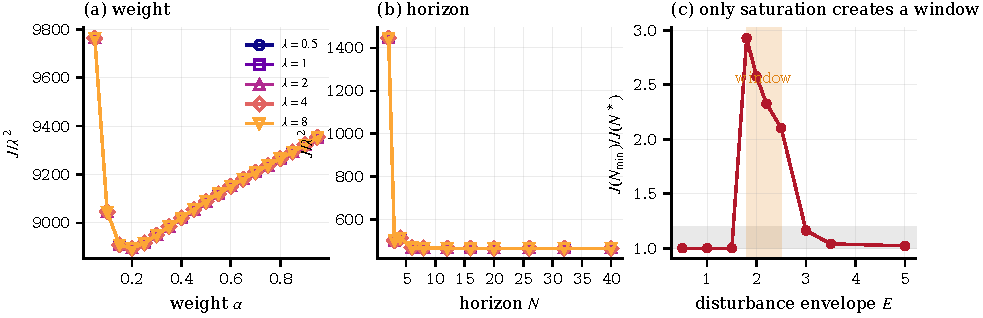
\includegraphics[width=\textwidth]{fig_scale.pdf}
\caption{Amplitude-scale invariance and its limit. (a,b) Normalized cost
$J/\lambda^2$ against weight and horizon for five disturbance scales, both
optima interior ($\alpha^\star=0.20$, $N^\star=32$): the curves coincide.
(c) With a saturating actuator a level-dependent optimum does appear, but only
in a narrow window of the disturbance envelope.}
\label{fig:scale}
\end{figure*}

\subsection{The graph field is an LTI filter bank, with a scope warning}
\begin{proposition}\label{prop:lti}
With $b=\beta=0$ in \eqref{eq:operators}, the map from the injected signal
$h_d$ to the node values $h$, in either branch, is linear and time invariant:
each node's response is the convolution of the source with a fixed impulse
response. (Verified to $1.1\times10^{-15}$ by superposition, exactly by time
invariance, and to $4.4\times10^{-16}$ by convolution reconstruction.)
\end{proposition}

Whatever the field contributes over the signal entering at the source is
therefore a fixed linear reshaping --- delay plus spreading. Two honest
caveats, both of which we got wrong before getting them right. First, the field
belongs to the class of LTI banks of order $2M$; a rival parametrizing that
whole class would contain it, but the seven-parameter shaped delay we use in
Section~\ref{sec:transport} does \emph{not}: measured on interior hops of an
eight-node chain, the field's kernels broaden with hop count, by a factor
that depends on the width measure used, at the operating point as well as at
nominal parameters. The field's defeat there is an empirical
finding, not a corollary. Second, the deployed governor is \emph{not} LTI ---
between $h$ and the applied meta-parameter sit a saturation, a projection onto
$\mathcal{A}$, and a quantizer --- and the reach law below depends on the
quantizer.

\subsection{The forcing decides whether anything crosses}
\begin{proposition}\label{prop:dc}
Take the forcing $f(h_d)=Kh_d$, so the stiffness term reads $-K(h-h_d)$ and
each node relaxes to its own target. Then the equilibrium is $h=h_d$ exactly,
$H(0)=K^{-1}K=I$, and the cross-node DC gain is identically zero: a sustained
alert injected at one node reaches no other node, under any tuning. With
$f(h_d)=\omega_0^2h_d$ the equilibrium is $\omega_0^2K^{-1}h_d$, whose
off-diagonal entries are nonzero, and with $G=0$ both branches share the same
$H(0)$, preserving the mechanism null.
\end{proposition}

A unit step at node~1 of a six-node chain settles to $[1,0,0,0,0,0]$ to
machine precision under the first forcing (Fig.~\ref{fig:dcgain}); only edges
cross, as transients. Our transport experiment originally asked the field to
deliver a sustained window under exactly this forcing --- the one thing its
structure forbids --- and the field's tuned gains pinned themselves to the top
of every grid trying to compensate, which was the observable symptom.

\begin{figure*}[t]
\centering
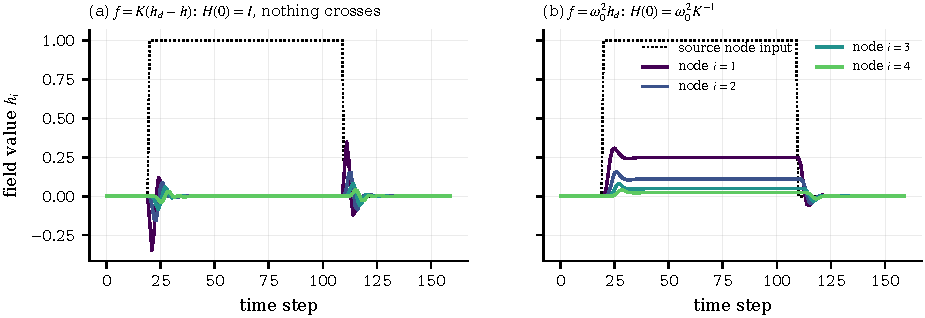
\includegraphics[width=\textwidth]{fig_dcgain.pdf}
\caption{Proposition~\ref{prop:dc}. (a) Under the homeostatic forcing the DC
transfer is the identity: a sustained input at the source produces nothing at
any other node. (b) Under the source forcing the sustained component crosses,
identically in both branches when $G=0$.}
\label{fig:dcgain}
\end{figure*}

\begin{observation}[Quantization-limited reach]\label{obs:reach}
If the closed-loop transported amplitude decays geometrically with hop count,
$a_n=a_0\rho^{\,n}$, and the meta-parameter moves only when that amplitude
exceeds one grid step $\Delta$, the reach is
$n_{\max}=\lfloor\log\Delta/\log\rho\rfloor$: logarithmic in the resolution of
the meta-parameter.
\end{observation}

Measured on an eight-node chain with $\rho=0.358$ fitted on interior nodes,
the step law matches at three of four resolutions and overpredicts by one
hop at $\Delta=0.005$ --- the third of the four, not the finest, which it
gets right. At that resolution the geometric law puts the disputed hop's
amplitude at $0.0059$ against a step of $0.005$: a fifth of a step above
threshold, so a single quantization event decides it
(Fig.~\ref{fig:quantization}). We report the pre-registered verdict as the
script recorded it --- the law is \emph{not} validated, four resolutions
being too few to call one miss a coincidence. Two cautions we needed: the reach is
an integer, so plotting the continuous expression against integer measurements
makes a correct law look wrong; and the terminal node of a chain has degree
one and retains signal, so fitting $\rho$ through it biases the estimate ---
an artifact that, we admit, also contaminated one of our own intermediate
re-measurements before we excluded terminal nodes throughout. The half-step
threshold that round-to-nearest quantization suggests fits none of the four
resolutions; the amplitude we report is a dispersion along the trace, not a
peak, and the empirical criterion is the full step.

\begin{figure*}[t]
\centering
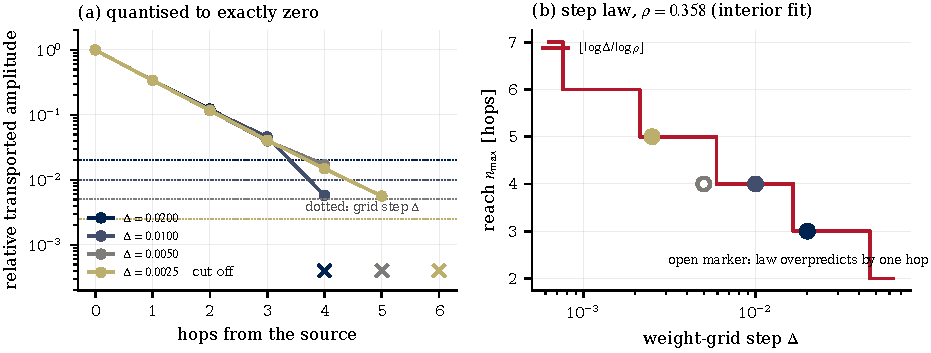
\includegraphics[width=\textwidth]{fig_quantization.pdf}
\caption{Observation~\ref{obs:reach}. (a) Transported amplitude against hop
count for four grid resolutions; crosses mark nodes quantized to exactly zero,
dotted lines the grid step. (b) Measured reach against grid step, with the step
law and $\rho=0.358$ fitted on interior nodes; the open marker is the one
resolution where the law overpredicts by a hop.}
\label{fig:quantization}
\end{figure*}

% ====================================================================
\section{Result I: Constant Anticipation, Not Proportional Delay}
\label{sec:transport}
% ====================================================================
The one use of a graph field that the structural limits leave open is
transport: a disturbance that travels physically downstream, so that the
upstream neighbour holds information about the downstream node's future which
no local horizon can obtain. Node $i$ experiences the source disturbance
delayed by $i\tau$ steps ($\tau=6$ in our chain of four nodes).

\subsection{Three viability filters}
Three checks preceded any comparison, each able to kill the arena. Without a
storage state, the lead sweep is flat: a nominal regulator at rest applies
$u^\star=0$ for every meta-parameter value, so advance warning has no channel
to act through --- unless the governor itself has lag, which is why we state
this as a filter rather than a theorem. With storage --- two objectives at
different setpoints, so the weight selects the buffer level and anticipating
means charging early --- anticipation buys $+4.0\%$ over the ideal reactive
limit ($t=+5.80$, $p=2.6\times10^{-4}$, nine of ten seeds, tuning and
evaluation seeds disjoint). The useful lead is short, two to four steps across
the physical range, and grows with actuator sluggishness as the mechanism
predicts.

\subsection{The discovery: our unreachable oracle was implementable}
We compared delivery mechanisms for the source measurement: an ideal local
detector (learns of the event the instant it arrives --- stronger than any
realizable detector), a per-hop delay line $k_i=\delta i$, the wave field, a
shaped delay (per-hop delay plus a second-order stage, matched to the field's
seven parameters), and, as a reference ceiling, a ``clairvoyant oracle'' that
opens a gate a fixed lead before each arrival.

Getting this comparison honest took three corrections, described in
Section~\ref{sec:methodology}; here is the one that produced the result. After
the causality guard was in place, the tuned oracle --- supposedly an
unreachable bound --- opened its gates a fixed number of samples ahead of
each arrival at every node, and never before the source measured. It was causal, and it was
reproduced \emph{exactly} (difference $0.0$) by a delay line
\begin{equation}
k_i=\max\{0,\ \tau i-\ell\},
\label{eq:affine}
\end{equation}
affine in the hop index with a constant anticipation term $\ell$. The
competition had excluded the best member of its own family. The proportional
family $k_i=\delta i$ cannot express \eqref{eq:affine}: with $\delta=\tau$ the
anticipation is zero everywhere, and with $\delta<\tau$ it grows with distance,
so far nodes are warned too early and near nodes too late. What the physics
supplies is anticipation \emph{growing} with distance ($i\tau$); what the loop
needs is anticipation \emph{constant} across nodes (saturated, for near nodes,
at the maximum physically available); the constant term is the conversion
between the two.

\subsection{The result}
Table~\ref{tab:transport} and Fig.~\ref{fig:transport} give the final
comparison: thirty evaluation seeds disjoint from the three tuning seeds,
causality guard active inside the tuning loop, causal (parameter-only)
normalization, equal tuning-grid densities for all mechanisms, and every tuned optimum
interior to its grid with one declared exception: the proportional family's
high weight lands on $a_{\mathrm{hi}}=1$, the top of the simplex, which is a
physical limit and not a grid artifact --- and it is the \emph{rival} whose
optimum sits there, so the exception does not favour our mechanism. The
archived sweep records the boundary status of every tuning, and the build
check re-reads it. The acausal reference itself sits at both simplex limits
($a_{\mathrm{lo}}=0$, $a_{\mathrm{hi}}=1$) by construction: it is a reference,
not a tuned mechanism, and the rule does not apply to it. The genuinely
acausal ceiling uses per-node anticipation beyond what the source can
supply and is labelled as a reference, not a mechanism and not a bound:
a causal mechanism turned out to reach it, which is the point of
Section~\ref{sec:transport}.

\begin{table}[t]
\caption{Transport chain, $30$ evaluation seeds. ``MDE'' is the minimum
detectable effect at power $0.8$ for the paired contrast; contrasts are
Holm-corrected \cite{holm1979}. The affine delay against the proportional
family's \emph{best known} tuning (from a denser grid, archived) still gives
$t=+5.40$, so the decisive contrast does not depend on the rival's version.}
\label{tab:transport}
\centering
\small
\setlength{\tabcolsep}{4pt}
\begin{tabular}{lrrr}
\toprule
mechanism & cost (s.e.m.) & vs.\ local & \% ceiling\\
\midrule
acausal ceiling            & $48\,944$ $(2828)$ & $+13.7$ & $100.0$\\
affine + shaping (7 par.)  & $49\,455$ $(2175)$ & $+12.8$ & $93.4$\\
\textbf{affine delay (4 par.)} & $\mathbf{49\,650}$ $(2370)$ & $\mathbf{+12.4}$ & $\mathbf{90.9}$\\
wave field (7 par.)        & $51\,054$ $(2083)$ & $+9.9$  & $72.8$\\
proportional delay (3 par.)& $51\,711$ $(2479)$ & $+8.8$  & $64.3$\\
ideal local detection      & $56\,690$ $(1301)$ & $0.0$   & $0.0$\\
\midrule
\multicolumn{4}{@{}l}{\textit{paired contrasts, Holm; $\delta$, $t$, $p$, MDE as \% of cost}}\\
affine vs.\ proportional & \multicolumn{3}{r}{$+2060$,\ $t{=}{+}17.87$,\ $p{<}10^{-4}$\,*,\ $0.6\%$}\\
affine vs.\ wave field   & \multicolumn{3}{r}{$+1403$,\ $t{=}{+}4.64$,\ $p{=}0.0002$\,*,\ $1.5\%$}\\
shaping the affine       & \multicolumn{3}{r}{$-195$,\ $t{=}{-}0.97$,\ $p{=}0.34$,\ $1.0\%$}\\
affine vs.\ local        & \multicolumn{3}{r}{$+7040$,\ $t{=}{+}6.29$,\ $p{<}10^{-4}$\,*,\ $5.5\%$}\\
ceiling vs.\ affine      & \multicolumn{3}{r}{$+706$,\ $t{=}{+}1.49$,\ $p{=}0.29$,\ $2.3\%$}\\
\bottomrule
\end{tabular}
\end{table}

\begin{figure*}[t]
\centering
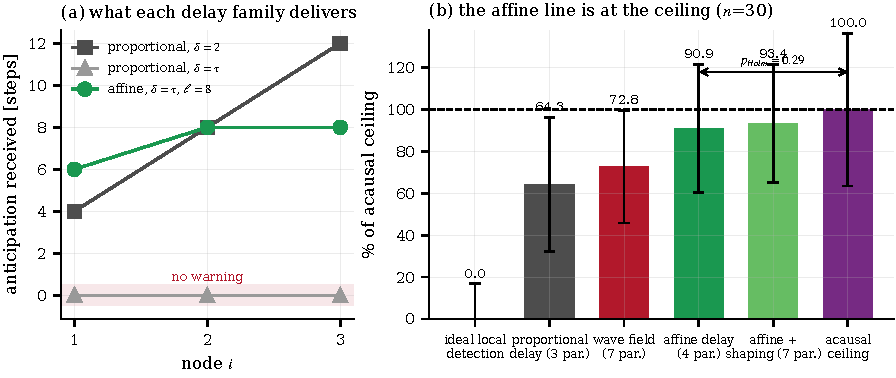
\includegraphics[width=\textwidth]{fig_transport.pdf}
\caption{(a) Anticipation received by each node under the two delay families:
the proportional family either wastes the near nodes' information or floods the
far nodes early; the affine family delivers constant anticipation, saturated at
what is physically available. (b) Final comparison, thirty seeds, error bars
one s.e.m.: the affine delay is within $-0.3\%$ to $+3.7\%$ ($95\%$
interval) of the acausal reference, and neither shaping nor the wave field
improves on it.}
\label{fig:transport}
\end{figure*}

Three readings. Having upstream information is worth $12.4\%$ against the best
possible local detector, and the study can resolve effects an order of
magnitude smaller than that. The \emph{structure} of delivery decides:
affine beats proportional at $t=+17.87$ under equal tuning densities, and at
$t=+5.40$ even against the proportional family's best tuning from a denser
grid. And nothing richer helps: adding the second-order shaping stage changes
nothing resolvable ($t=-0.97$ against an MDE of $1.0\%$), the wave field is
significantly worse than the plain affine line ($t=+4.64$), and the affine line
is within $-0.3\%$ to $+3.7\%$ of the acausal reference ($95\%$
interval; it is cheaper than the reference in $13$ of
$30$ seeds, paired $t=+1.49$, raw $p=0.15$,
Holm $p=0.29$; MDE $2.3\%$ --- an equivalence bound, not a proof of
optimality). Resampling the thirty paired seeds puts
the recovered fraction at $90.9\%$ with a $95\%$ interval of
$[84.9,103.9]$, and in $6.3\%$ of the resamples the causal line is \emph{cheaper}
than the acausal reference. That is why we report a reference rather than a
bound: a quantity a causal mechanism can beat six times in a hundred is not
bounding anything. We state the one asymmetry that survives:
the field's kernel does differ across hops (Proposition~\ref{prop:lti}
discussion), so its defeat is empirical, bounded by these MDEs, not
structural.

% ====================================================================
\section{Result II: A Certificate Detector Governing the Horizon}
\label{sec:alphaN}
% ====================================================================
\subsection{Single loop: the frontier, and who sits below it}
We first close the loop $\alpha_t\rightarrow$ governor $\rightarrow N_t$ on a
single plant, with pre-registered hypotheses, ten seeds, and computation
accounted honestly: every QP is charged, including those used to measure
$\alpha_t$, with the instrument solve reused as the next control solve when the
horizon does not change. Table~\ref{tab:alphaN} reports the out-of-envelope
scenario (larger kicks plus model mismatch) against the frontier traced by
fixed horizons at equal computation.

\begin{table}[t]
\caption{Horizon governance, out-of-envelope scenario, ten seeds. Computation, cost
and assignment correlation are means over the seeds that did \emph{not}
diverge; the last column counts the divergences. Divergent runs are also
excluded pairwise from the contrasts; the $N=2$
row's computation and cost are means over a run set with half the seeds dead,
and are shown for completeness rather than comparison.}
\label{tab:alphaN}
\centering
\small
\setlength{\tabcolsep}{4pt}
\begin{tabular}{@{}lrrcc@{}}
\toprule
governor & comput. & cost & corr & div.\\
\midrule
fixed $N=2$                    & $610$  & $29653$ & --- & $5$\\
fixed $N=4$                    & $1600$ & $12561$ & --- & $0$\\
fixed $N=6$                    & $2400$ & $12124$ & --- & $0$\\
fixed $N=8$                    & $3200$ & $12104$ & --- & $0$\\
fixed $N=16$                   & $6400$ & $12103$ & --- & $0$\\
\midrule
\textbf{leaky integrator}      & $\mathbf{1775}$ & $\mathbf{12211}$ & $0.935$ & $0$\\
threshold                      & $3051$ & $12103$ & $0.858$ & $0$\\
2nd-order field ($\zeta{=}0.5$)& $3133$ & $17862$ & $0.270$ & $2$\\
memoryless map                 & $3666$ & $27620$ & $0.367$ & $5$\\
\bottomrule
\end{tabular}
\end{table}

Interpolating the frontier at the leaky integrator's $1775$ units gives
roughly $12\,470$; the governor achieves $12\,211$, about $2\%$ below the
frontier, without knowing the correct horizon in advance. The second-order
field rings --- it drops the horizon mid-recovery, breaks the certificate
again and re-excites itself; critical damping repairs its assignment
correlation in the large-kick scenario ($-0.42$ to $+0.43$, $t=+7.26$), which
identifies ringing as the mechanism, but a critically damped second-order
filter is a first-order filter with extra lag and does not beat one. On
assignment correlation the leaky integrator is best in two of the four
scenarios, including both out-of-envelope kick scenarios (with and without
model mismatch). What broke
out-of-envelope was not short \emph{fixed} horizons at moderate $N$ ---
replanning compensates from $N=4$ up, though $N=2$ does diverge on half the
seeds --- but short-\emph{memory adaptive} governors, which under-assign right
after a kick. The risk is aggressive downward modulation, not a modest fixed
horizon.

The demand signal $\alpha_t$ generates is a pulse train; the natural decoder
of pulse durations is a leaky integrator, not a resonator. Pushing the
governor's reference toward zero turned out to improve it monotonically, with
a plateau at the limit: the optimal governor is a \emph{detector of certificate
violation} --- request $N_{\max}$ when $\alpha_t\le0$, request $N_{\min}$
otherwise --- behind a slow leak ($\tau=30$ samples in the fleet;
the single-loop bank of Table~\ref{tab:alphaN} ran with $\tau=14.7$ and
$a_{\mathrm{ref}}=0.6$, and is therefore not this detector limit). Two effective
parameters, and the event it reacts to is the one event in the signal with a
meaning in the theory \cite{gruene2017nmpc}.

\subsection{A fleet sharing one embedded controller}
A factor-two saving in computation matters most where predictive control is
most constrained: one embedded controller serving many loops, the sampling
period fixing a hard computation budget per step. We model $M=8$ thermal
collector loops (fluid state coupled to a slower absorber,
$\tau_f=2$\,min, $\tau_m=5$\,min, $dt=30$\,s), with cloud-passage disturbances
and a knob $\rho$ setting the fraction that sweeps all loops at once. The
penalized variable is the \emph{absorber} temperature, which the flow reaches
only through the fluid; without that delay between action and effect the bench
is empty --- penalizing the directly actuated state leaves the fixed-horizon
frontier flat in $N$ and nothing to govern, against a ratio
$J(N{=}2)/J(N{=}16)=1.47$ here.

Two accounting disciplines decide whether this comparison means anything, and
we broke both before fixing them (Section~\ref{sec:methodology}). The budget
must bind on computation actually \emph{spent} --- including the certificate
measurement --- not on horizons granted; and the governor must be \emph{tuned}
under the same accounting it is evaluated under. With both in place, the rival
is the fixed-horizon frontier interpolated, per seed, at the governor's real
computation; interpolation between adjacent integer horizons is achievable by
alternating horizons between steps, so it concedes nothing.

\begin{table}[t]
\caption{Fleet of $M=8$ loops, eight evaluation seeds disjoint from the three
tuning seeds. Governor tuned by a grid sweep archived with the script, under the
evaluation metric itself ($\tau=30$, interior to the grid; reference
$a_{\mathrm{ref}}\to0$, the certificate-detector limit, on a plateau whose
dispersion below $0.03$ is $0.65\%$). Cost against the fixed-horizon frontier at equal spent
computation, paired per seed against that seed's own frontier. The $B=16$ row
is degenerate: every loop is pinned at $N_{\min}$.}
\label{tab:fleet}
\centering
\small
\setlength{\tabcolsep}{3.6pt}
\begin{tabular}{@{}crrrr@{}}
\toprule
$B/(MN_{\max})$ & spent & governed & frontier & change\\
\midrule
\multicolumn{5}{@{}l}{\textit{independent disturbances} ($\rho=0$)}\\
$0.19$ & $26.0$ & $2814$ & $2993$ & $\mathbf{-6.0\%}$\,*\\
$0.25$ & $35.2$ & $2567$ & $2732$ & $\mathbf{-6.0\%}$\,*\\
$0.31$ & $41.1$ & $2470$ & $2598$ & $-4.9\%$\,*\\
$0.38$ & $42.9$ & $2443$ & $2568$ & $-4.9\%$\,*\\
$\ge0.50$ & $43.1$ & $2440$ & $2564$ & $-4.8\%$\,*\\
\midrule
\multicolumn{5}{@{}l}{\textit{common front} ($\rho=1$)}\\
$0.19$ & $23.8$ & $4589$ & $4599$ & $-0.2\%$\phantom{\,*}\\
$0.25$ & $29.1$ & $4208$ & $4343$ & $-3.1\%$\,*\\
$0.31$ & $33.5$ & $3912$ & $4149$ & $\mathbf{-5.7\%}$\,*\\
$0.38$ & $37.3$ & $3750$ & $4003$ & $\mathbf{-6.3\%}$\,*\\
$0.50$ & $43.1$ & $3645$ & $3829$ & $-4.8\%$\,*\\
$0.75$ & $48.2$ & $3638$ & $3716$ & $-2.1\%$\phantom{\,*}\\
$1.00$ & $48.3$ & $3638$ & $3715$ & $-2.1\%$\phantom{\,*}\\
\bottomrule
\end{tabular}
\end{table}

Table~\ref{tab:fleet} and Fig.~\ref{fig:fleet}: with independent disturbances
the governor beats the best fixed horizon at equal spent computation at every
budget that binds --- seven of the eight rows, of which the three loosest are
one experiment, since the governor saturates at the same spent computation ---
by up to $6.0\%$ (Holm-adjusted $p<10^{-4}$ throughout); under a
perfectly correlated front it wins at 4 of eight budgets after Holm
adjustment, by up to $6.3\%$, and the two loosest budgets favour it by
$2.1\%$ at raw $p<0.03$ but not after adjustment
($p=0.073$). Under independence the advantage is largest where the
budget binds and settles at $4.8\%$ once it stops binding; under a
common front it is concentrated in mid-range budgets and vanishes at both
ends. The eighth budget, $B=16$ ($0.125$), is omitted from the table: every
loop is pinned at $N_{\min}$ and the two arms coincide to $0.03\%$.

The decomposition in Fig.~\ref{fig:fleet}(b) separates the two mechanisms
with one arm each, and it corrected our own reading of them. \emph{Allocation}
is isolated by keeping the governor and its temporal adaptation --- the same
total horizon per step --- and only distributing it equally instead of in
proportion to demand; \emph{timing} is isolated by comparing that
equal-split governed arm against a fixed horizon at equal spent computation.
The two components turn out to be complementary rather than cumulative.
Allocation pays $+6.1\%$ to $+7.1\%$ when disturbances
are independent (all six budgets at equal spent computation, eight seeds each)
and next to nothing under a common front ($0.0\%$ to
$+1.4\%$, significant after Holm at 2 of six budgets):
with every loop in trouble at once there is no one to take horizon from.
Timing does the opposite --- it pays $+2.2\%$
to $+5.2\%$ under a common front at
the 4 middle budgets, where the moment to spend is well defined,
and nothing at the tightest and loosest; under independence it is not merely
neutral but \emph{harmful}, down to $-3.7\%$: with someone always
in trouble the aggregate demand is nearly constant, so modulating it in time
only mistimes the spending that the allocation arm then has to repair. Each
regime is carried by one mechanism, which is why the governor wins in both.

\begin{figure*}[t]
\centering
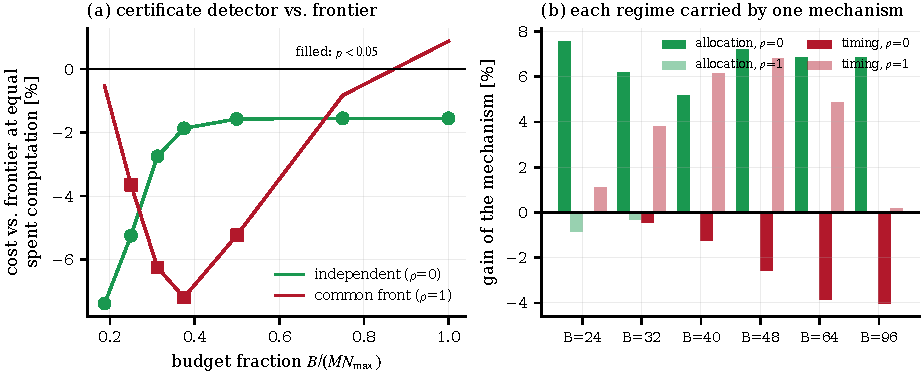
\includegraphics[width=\textwidth]{fig_fleet.pdf}
\caption{(a) Fleet cost against the fixed-horizon frontier at equal
\emph{spent} computation, for independent and perfectly correlated
disturbances: the certificate-detector governor wins across budgets in both.
(b) Decomposition into its two mechanisms, each isolated by one arm:
allocation (demand-proportional versus equal-split, same governor and same
total horizon per step) and timing (equal-split governed versus fixed
horizon, at equal spent computation). They are complementary: allocation
pays only under independence, timing only under a common front --- up to
$+5.2\%$ --- and timing is actively harmful under
independence.}
\label{fig:fleet}
\end{figure*}

% ====================================================================
\section{The Arena Map}\label{sec:arenas}
% ====================================================================
Table~\ref{tab:arenas} summarizes the six arenas. The one the field won is the
one whose demand was an exogenous priority signal with no physical origin, and
we do not count it as evidence.

\begin{table}[t]
\caption{The six arenas. ``Demand'' is the signal the governor is asked to
track.}
\label{tab:arenas}
\centering
\small
\begin{tabular}{p{1.45cm}p{1.85cm}p{3.8cm}}
\toprule
arena & demand & outcome\\
\midrule
synthetic weights & exogenous priority, no physics & field wins out of
distribution; no physical origin, not counted\\
greenhouse price & smooth, clean & modulation loses; the horizon already
arbitrates the price\\
graph, shared price & global signal & no gain: sharing what is already
common\\
$\alpha_N$ horizon & pulse train & pays; certificate detector + leak wins,
the field rings\\
narrow-band vibration & postulated from absolute amplitude & loses $8/8$
to a per-condition re-optimized constant; quartic metric, outside
Proposition~\ref{prop:scale}\\
transport, storage & travelling event & pays $12.4\%$; affine delay wins,
field and shaping add nothing\\
\bottomrule
\end{tabular}
\end{table}

\begin{figure}[t]
\centering
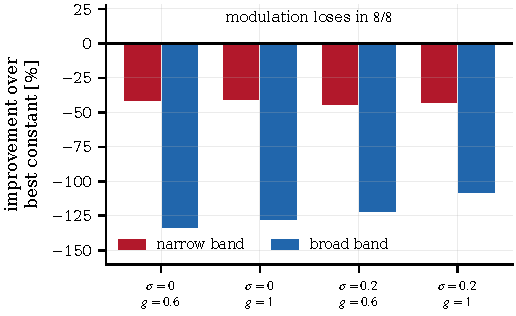
\includegraphics[width=\columnwidth]{fig_vibration.pdf}
\caption{The narrow-band arena, built expressly to favour the field: resonant
structure, beat disturbance, fatigue cost, and a schedule
$\alpha_d=1/(1+\kappa E^2)$ \emph{derived} from that cost. It loses in all
eight configurations against a per-condition re-optimized constant weight,
which already absorbs the amplitude dependence the schedule was built to
supply. The fatigue metric is quartic, so this arena lies outside
Proposition~\ref{prop:scale}: the defeat is empirical, not a
corollary.}
\label{fig:vibration}
\end{figure}

There is a tension worth stating plainly, because it bounds future attempts.
For modulation to pay one must cross a nonlinearity; crossing one makes the
demand eventual, hence broadband, which is the regime where a leak beats a
resonator. For inertia to pay one wants narrow-band demand, whose canonical
manufacture is amplitude modulation, which Proposition~\ref{prop:scale} strips
of absolute-amplitude content. The two conditions an inertial governor needs
sit awkwardly together, and in six arenas they never met.

% ====================================================================
\section{Five Leaks, and the Tests That Now Guard Them}
\label{sec:methodology}
% ====================================================================
Every arena above was first decided by a defect rather than by its
mechanisms. We document the five that form a pattern. None of them is exotic;
each is the kind of line a careful person writes without noticing, and each
has a mechanical guard cheap enough to run inside a tuning loop. Table~\ref{tab:audit} lists the
resulting suite.

\paragraph{Leak 1: a broken channel (DC cross-gain)}
The field was first run with the homeostatic forcing, whose cross-node DC gain
is identically zero (Proposition~\ref{prop:dc}); the experiment asked it to
deliver a sustained window, the one signal it cannot carry, and the field lost
to a trivial delay line. The symptom was tuned gains pinned to grid
boundaries. \emph{Guard:} probe the channel with a sustained step and measure
what arrives, before comparing anything (assertion A18).

\paragraph{Leak 2: an acausal time shift}
A free time-shift in the signal-conditioning stage is a natural knob to
include in a tuning grid; if the grid contains negative values, it silently
hands the mechanism information from the future. Both leading mechanisms took
the option --- their gates opened up to eight steps before the source measured
the event --- and the only fair player was the simplest rival. The headline
contrast of that version ($t=+5.45$) dissolved to $t=+0.05$ under the guard.
\emph{Guard:} a single-pulse probe inside the tuning loop; reject any
configuration whose output moves before the input does.

\paragraph{Leak 3: an acausal normalization}
The map from field value to weight was normalized by the trace's min and max
--- computed over the \emph{whole} trace, so the scale at time $t$ depended on
the future. Truncating the trace after the event measurably changed the gate
\emph{before} the event. Only the two seven-parameter mechanisms
used the normalization; the delay line did not. \emph{Guard:} the truncation
probe --- run the mechanism on the full and on a truncated input; on the
shared prefix the outputs must agree exactly. This test requires no hypothesis
about where the leak is, which is how it caught one we did not suspect. The
fix (normalizing by the DC gain, a pure function of parameters) also removed a
free knob.

\paragraph{Leak 4: budget granted versus computation spent}
The fleet's budget bound the horizons \emph{granted}, while the governor also
spent computation measuring its certificate; it consumed $18$--$26\%$ more
than the fixed rival at the same nominal budget, and ``won'' by
overspending. \emph{Guard:} account computation where it is spent and compare
on the (spent, cost) plane. The single-loop experiment already did this; the
fleet inherited the budget from the wrong side of the ledger.

\paragraph{Leak 5: tuning under one metric, evaluating under another}
After fixing Leak~4 we re-tuned the governor by raw cost at fixed nominal
budget --- a criterion that still rewards overspending --- and it moved the
optimum to a faster leak and shrank the advantage at every budget that did not
bind. Tuned under the evaluation metric itself (the gap to the per-seed
frontier at spent computation, summed over the tuning budgets), the optimum
returns to the slow leak and the governor wins by up to $6\%$. This
leak is the mirror image of the others: it \emph{deflated} the result it
touched, and it did so twice --- the tuning script of an earlier revision still
used raw cost while the text claimed otherwise, which an adversarial review of
the script, not of the text, caught. Leaks do not consistently favour the pet
mechanism; they favour whatever the criterion mismatch happens to favour, which
is why the guard must be mechanical. \emph{Guard:} the tuning objective must
be the evaluation metric, computed the same way.

\paragraph{Three disciplines, used throughout}
Reject any tuned optimum on the boundary of its grid, with the exception of
physical limits (a weight saturating at the simplex boundary is not a grid
artifact) --- applied to ourselves twice, including once to the evidence for
Proposition~\ref{prop:scale}. Report, with every null contrast, the minimum
detectable effect: ``no difference'' in Table~\ref{tab:transport} means
``bounded by the stated MDE,'' never ``proved zero.'' And treat an
``unreachable'' bound that a guard fails to disqualify as a finding: our
oracle passed the causality guard --- assertion A19 re-runs that probe on
the published tuning rather than only inside the sweep --- which is how we
learned the competitor
family was mis-specified (Section~\ref{sec:transport}).

\begin{table}[t]
\caption{Executable audit suite: $21$ checks over $19$ assertions (A9 runs at
three damping ratios). Each encodes a defect found at least once.}
\label{tab:audit}
\centering
\small
\begin{tabular}{@{}l@{\ }p{6.3cm}@{}}
\toprule
id & assertion\\
\midrule
A1--A3 & terminal inequality, invariance of $\Omega$, constraint
         satisfaction\\
A4--A5 & $\vstar(x,\cdot)$ concave in $\alpha$; admissible set can be
         non-convex\\
A6 & the certified radius is valid\\
A7 & first/second-order matching is exact \emph{in discrete time}\\
A8 & anti-windup does not fire when nothing is blocked\\
A9 & executed overshoot equals that of the \emph{discrete} system\\
A10--A11 & gyroscopic collocation stable; Merkin threshold\\
A12 & the inherited terminal ingredient fails (documented regression)\\
A13--A14 & monotonicity duality of $V_N$ in $N$\\
A15 & scale invariance: normalized cost \emph{curves} coincide; fails on
      boundary optima (Prop.~\ref{prop:scale})\\
A16 & anticipation unusable without storage (viability filter)\\
A17 & the field with $\beta=0$ is exactly LTI (Prop.~\ref{prop:lti})\\
A18 & DC cross-gain of the two forcings (Prop.~\ref{prop:dc})\\
A19 & the causality guard bites at the \emph{published} tuning, and the
      clairvoyant reference fails it\\
\bottomrule
\end{tabular}
\end{table}

We record two calibration facts. Divergent runs are excluded pairwise and
reported as counts, because a run that dies early contributes a truncated sum
and ``wins'' computation by dying. And a contrast that moves from $t=+17.9$ to
$t=+5.4$ when the rival's tuning grid is densified, or from significant to
nothing when a guard is enforced, is a statement about the protocol, not the
mechanism; we report both values wherever that happened.

% ====================================================================
\section{Conclusions}\label{sec:conclusions}
% ====================================================================
We set out to show that a homeostatic wave field is a good distributed
governor for the meta-parameters of MPC, and it is not: in every physically
grounded arena it is beaten or matched by a minimal mechanism --- and the
margin by which we can bound the ties is stated with every claim.

What replaces it is a design lesson with two instances. Where a disturbance
travels, deliver its warning with \emph{constant} anticipation: an affine
delay line, four parameters, within $-0.3\%$ to $+3.7\%$ of the acausal
clairvoyant reference, worth $12.4\%$ against the best local detection, with the proportional family that
per-hop designs default to significantly and explicably worse. Where a
horizon must be rationed, react to the one event in the suboptimality signal
that theory distinguishes --- the certificate breaking --- through a slow
leak: two effective parameters, below the fixed-horizon frontier in a single
loop, and up to $7\%$ ahead of the best fixed horizon in a fleet at equal
spent computation under either disturbance-correlation regime --- carried by
allocation when the loops fail at different times and by timing when they fail
together, each mechanism useless or harmful in the other's regime.

The structural limits say these are not accidents of tuning: nothing built on
absolute amplitude can carry information to a meta-parameter, an LTI field
offers reshaping rather than information, its natural forcing carries nothing
sustained at all, and quantization caps its reach logarithmically. And the
five leaks say something about practice that we did not expect to be the
paper's most durable contribution when we began: every one of our arenas was
first decided by a defect, the defects were ordinary, the guards are cheap,
and two of the five pushed the result \emph{against} the mechanism we were
defending. Honest comparisons are not a matter of intention; they are a
matter of instrumentation.

\section*{Reproducibility}
All experiments, figures and the audit suite are generated by archived
scripts. A checker, run by the authors before each submission (it is not part
of the \LaTeX{} build), regenerates $94$ reported quantities from their
result files and requires each to occur in the body of this document as a
standalone numeric token, anchored on both sides so that a stray $8$ does not
match inside $0.85$. Of the $157$ numeric literals in the body with three or
more digits or a decimal point, those $94$ are regenerated in this sense;
$56$ more coincide with some value stored in an archived result file, which is
a check of existence rather than of provenance; and $7$ are declared constants
that come from no experiment, such as postal codes and column widths. A
mutation test alters, one occurrence at a time, each of the $94$ regenerated
quantities and re-runs the whole checker; every such mutant is caught.
Literals of one or two digits, and the counts in this paragraph, are outside
that audit; the checker asserts the counts. Tuning and evaluation seeds are
disjoint in every experiment reported.

\section*{Acknowledgment}
The authors used Claude (Anthropic), a large language model accessed
through the Claude Code command-line assistant, in the preparation of
this article. Following the IEEE PSPB Operations Manual, the use is
disclosed here in the terms in which it occurred. \emph{Code.} The simulation and analysis code, the plotting scripts, the
numerical verifier and its mutation test were written with that
assistance, from the protocols, pre-registrations and acceptance criteria
specified by the authors, who ran them and are responsible for their
outputs. \emph{Text.} All sections were drafted and revised with the same
assistance; the authors rewrote and checked every passage and are
responsible for every claim it makes. \emph{Adversarial review.} The rounds of adversarial review referred to in the title
footnote and in the Introduction were carried out with
agents of the same system, directed at this manuscript, at its code and at
its archived results; the authors decided which findings to accept and
what to do about each. \emph{What is not AI-generated.} No datum reported here was produced,
simulated or emulated by an AI system: the reported quantities come from
executing the project's simulation code. No figure contains AI-generated
imagery and none was retouched by an AI system; the assistance is confined
to the plotting code. No AI system is an author of this article, and the
authors take full responsibility for its entire content.

\bibliographystyle{IEEEtran}
\bibliography{refs}

\end{document}
